\section{Implementación y Propuesta Arquitectónica}

Para que el Portal Agro-Comercial trascienda su estado actual de prototipo académico funcional y evolucione hacia una plataforma de misión crítica capaz de operar 24/7 en condiciones reales de mercado, es imperativo intervenir sus cimientos estructurales. La deuda técnica, aunque invisible en el corto plazo, constituye el principal obstáculo para la escalabilidad.

En esta sección se realiza una disección técnica exhaustiva del sistema. Primero, se presenta la radiografía del estado actual de operación en el municipio de Teruel (denominado estado ``As-Is''), evidenciando con precisión ingenieril sus fortalezas de diseño y sus limitaciones de despliegue. Posteriormente, se detalla la propuesta de ingeniería para la inyección del patrón de \textit{Feature Toggles} (estado ``To-Be''), aplicando principios de robustez, desacoplamiento y estrategias de caché identificados durante la fase de investigación.

\subsection{Línea Base: Arquitectura Actual del Portal (As-Is)}

El sistema que hoy se encuentra operativo en los servidores de producción no pretende reinventar la rueda, sino aplicar un pragmatismo tecnológico orientado a resolver un problema sociotécnico: la conectividad intermitente. Se optó por una arquitectura distribuida y desacoplada, priorizando una única meta de negocio: garantizar que el campesino pueda gestionar su oferta independientemente de la calidad de su red móvil.

\subsubsection{El Núcleo Transaccional (Backend Monolítico)}

En el ``cuarto de máquinas'', la lógica de negocio reside en un ecosistema Microsoft basado en \textbf{ASP.NET Core} y el ORM \textbf{Entity Framework}. La decisión de centralizar allí las reglas pesadas —como el algoritmo de asignación de pedidos, la normalización de direcciones veredales y la validación de unidades de medida agrícola— responde a la necesidad de blindar la integridad referencial de los datos (ACID) mediante un motor relacional \textbf{SQL Server}.

Esta capa actúa como la única fuente de verdad (\textit{Single Source of Truth}), exponiendo servicios RESTful estandarizados que son agnósticos al cliente que los consume. Sin embargo, su despliegue es monolítico: todos los controladores, servicios y repositorios se compilan en un único ensamblado (\texttt{.dll}). Esto implica que el dominio de ``Usuarios'' y el dominio de ``Productos'' están físicamente acoplados en el mismo proceso de memoria.

\subsubsection{Estrategia de Supervivencia Digital (Frontend SPA)}

La decisión más crítica se tomó en la capa de presentación. Se adoptó el framework \textbf{Angular} para construir una SPA (\textit{Single Page Application}), no por motivos estéticos sino por una decisión de supervivencia digital basada en la capacidad de almacenamiento local (\textit{IndexedDB} y \textit{LocalStorage}).

De esta manera, si la señal celular fluctúa en una vereda —una realidad cotidiana en la geografía quebrada del Huila—, el catálogo de productos no desaparece ni la sesión se cierra abruptamente. La interfaz permanece responsiva, permitiendo al usuario completar sus tareas en un estado ``offline'' y sincronizar los datos de manera transparente una vez se restablece la conexión.

\subsubsection{El Problema del Acoplamiento en el Despliegue}

A pesar de las virtudes mencionadas, esta arquitectura presenta un ``talón de Aquiles'': el fuerte acoplamiento en el ciclo de liberación. Actualmente, el proceso de actualización es altamente intrusivo. Si se desea optimizar el algoritmo de búsqueda o corregir un error tipográfico menor en el formulario de registro, el procedimiento exige:

\begin{enumerate}
    \item Detener el \textit{Application Pool} en el servidor (IIS/Kestrel).
    \item Reemplazar los binarios compilados.
    \item Reiniciar el servidor para recargar la memoria.
    \item Invalidar la caché del navegador de los usuarios.
\end{enumerate}

Estas ventanas de mantenimiento, aunque breves (5--10 minutos), interrumpen la operación comercial y erosionan la confianza del usuario, un lujo que una plataforma con proyección nacional no puede permitirse.

\input{tables/arquitectura_actual}

\subsection{Propuesta de Diseño: Arquitectura Orientada a Toggles (To-Be)}

La solución propuesta no implica la demolición del portal existente —lo cual sería económicamente inviable—, sino una evolución quirúrgica hacia una arquitectura dirigida por configuración. Siguiendo las heurísticas de \cite{ajmeri2022heuristics}, se ha diseñado un modelo donde los toggles no son simples sentencias \texttt{if/else} dispersas desordenadamente por el código, sino una capa de control transversal (\textit{Cross-Cutting Concern}) gestionada de forma centralizada.

\subsubsection{Arquitectura del Feature Manager}

El núcleo de la propuesta es la implementación de un \textbf{Feature Manager}, un servicio \textit{singleton} encargado de evaluar reglas de negocio en tiempo real. Este componente desacopla la decisión de activar una funcionalidad de su implementación.

A diferencia de una configuración estática (como un archivo \texttt{appsettings.json} que requiere reinicio), este gestor evalúa el contexto de cada petición HTTP. Para ello, se diseñó un esquema de base de datos relacional que soporta tres niveles de granularidad, alineados con la taxonomía de \cite{chen2025horizon}:

\begin{itemize}
    \item \textbf{Global Toggles:} Activan o desactivan una función para toda la plataforma (ej. ``Modo Mantenimiento'').
    \item \textbf{Segment Toggles:} Se activan según atributos del usuario (ej. ``Usuarios de la Cooperativa Coofisam'').
    \item \textbf{Identity Toggles:} Permiten la activación granular a nivel de usuario individual (ej. ``Beta Tester Juan Pérez'').
\end{itemize}

\subsubsection{Estrategia de Interceptación en Backend (.NET)}

Para la API, la estrategia técnica se fundamenta en la interceptación mediante polimorfismo e Inyección de Dependencias (DI). Se propone implementar el patrón \textit{Decorator} o utilizar \textit{Action Filters} en el pipeline de ASP.NET Core.

Siguiendo las recomendaciones de resiliencia de \cite{esther2025microservices}, supóngase el desarrollo de una nueva lógica de validación de stock (\texttt{NewStockValidator}) más estricta que la actual (\texttt{LegacyStockValidator}). Ambas versiones coexisten implementando la misma interfaz \texttt{IStockValidator}.

El contenedor de inyección de dependencias se configura para resolver una implementación \textit{Proxy}, la cual consulta al \textit{Feature Manager} en tiempo de ejecución:

\begin{itemize}
    \item Si el toggle \texttt{StockV2} está activo $\rightarrow$ se ejecuta \texttt{NewStockValidator}.
    \item Si el toggle está inactivo o el sistema de configuración falla $\rightarrow$ se ejecuta \texttt{LegacyStockValidator} (\textit{fallback} seguro).
\end{itemize}

Esto habilita lo que \cite{ramaswamy2024zerodowntime} denominan ``tiempo de inactividad cero'': revertir errores funcionales requiere únicamente desactivar una bandera, sin \textit{rollback} de despliegue ni reinicio del servidor.

% --- INICIO DEL BLOQUE DE IMAGEN ---
% Figura a doble columna para evitar que el texto se monte sobre el gr\u00e1fico.
\begin{figure*}[t]
    \centering
    \includegraphics[width=0.95\textwidth]{graphics/flujo_toggle_backend.png}
    \caption{Diagrama de flujo propuesto para el backend. El "Toggle Router" intercepta la petición y decide dinámicamente que versión de la logíca ejecutar basandose en la configuración externa, desacoplando el despliegue de la activación.}
    \label{fig:flujo_backend}
\end{figure*}
% --- FIN DEL BLOQUE DE IMAGEN ---


\subsubsection{Optimización Frontend con Carga Condicional (Angular)}

En el cliente web, la prioridad es la optimización del ancho de banda y la memoria del dispositivo. Se descarta la práctica superficial de ``ocultar componentes con CSS'' (\textit{Feature Hiding}), ya que continúa descargando código innecesario.

Se propone una carga perezosa real (\textit{Conditional Lazy Loading}) mediante \textit{Route Guards} y módulos de Angular:

\begin{enumerate}
    \item La aplicación descarga un ``Manifiesto de Features'' (JSON liviano).
    \item El \textit{Router} de Angular consulta este manifiesto antes de cada navegación.
    \item Si el toggle ``Mapa Interactivo V2'' está inactivo, se bloquea la descarga del \textit{chunk} correspondiente.
\end{enumerate}

Con ello, las librerías pesadas de geolocalización no viajan por la red móvil, alineándose con las recomendaciones de optimización de interfaces dinámicas de \cite{lee2025frontend}.

\begin{figure}[htbp]
    \centering
    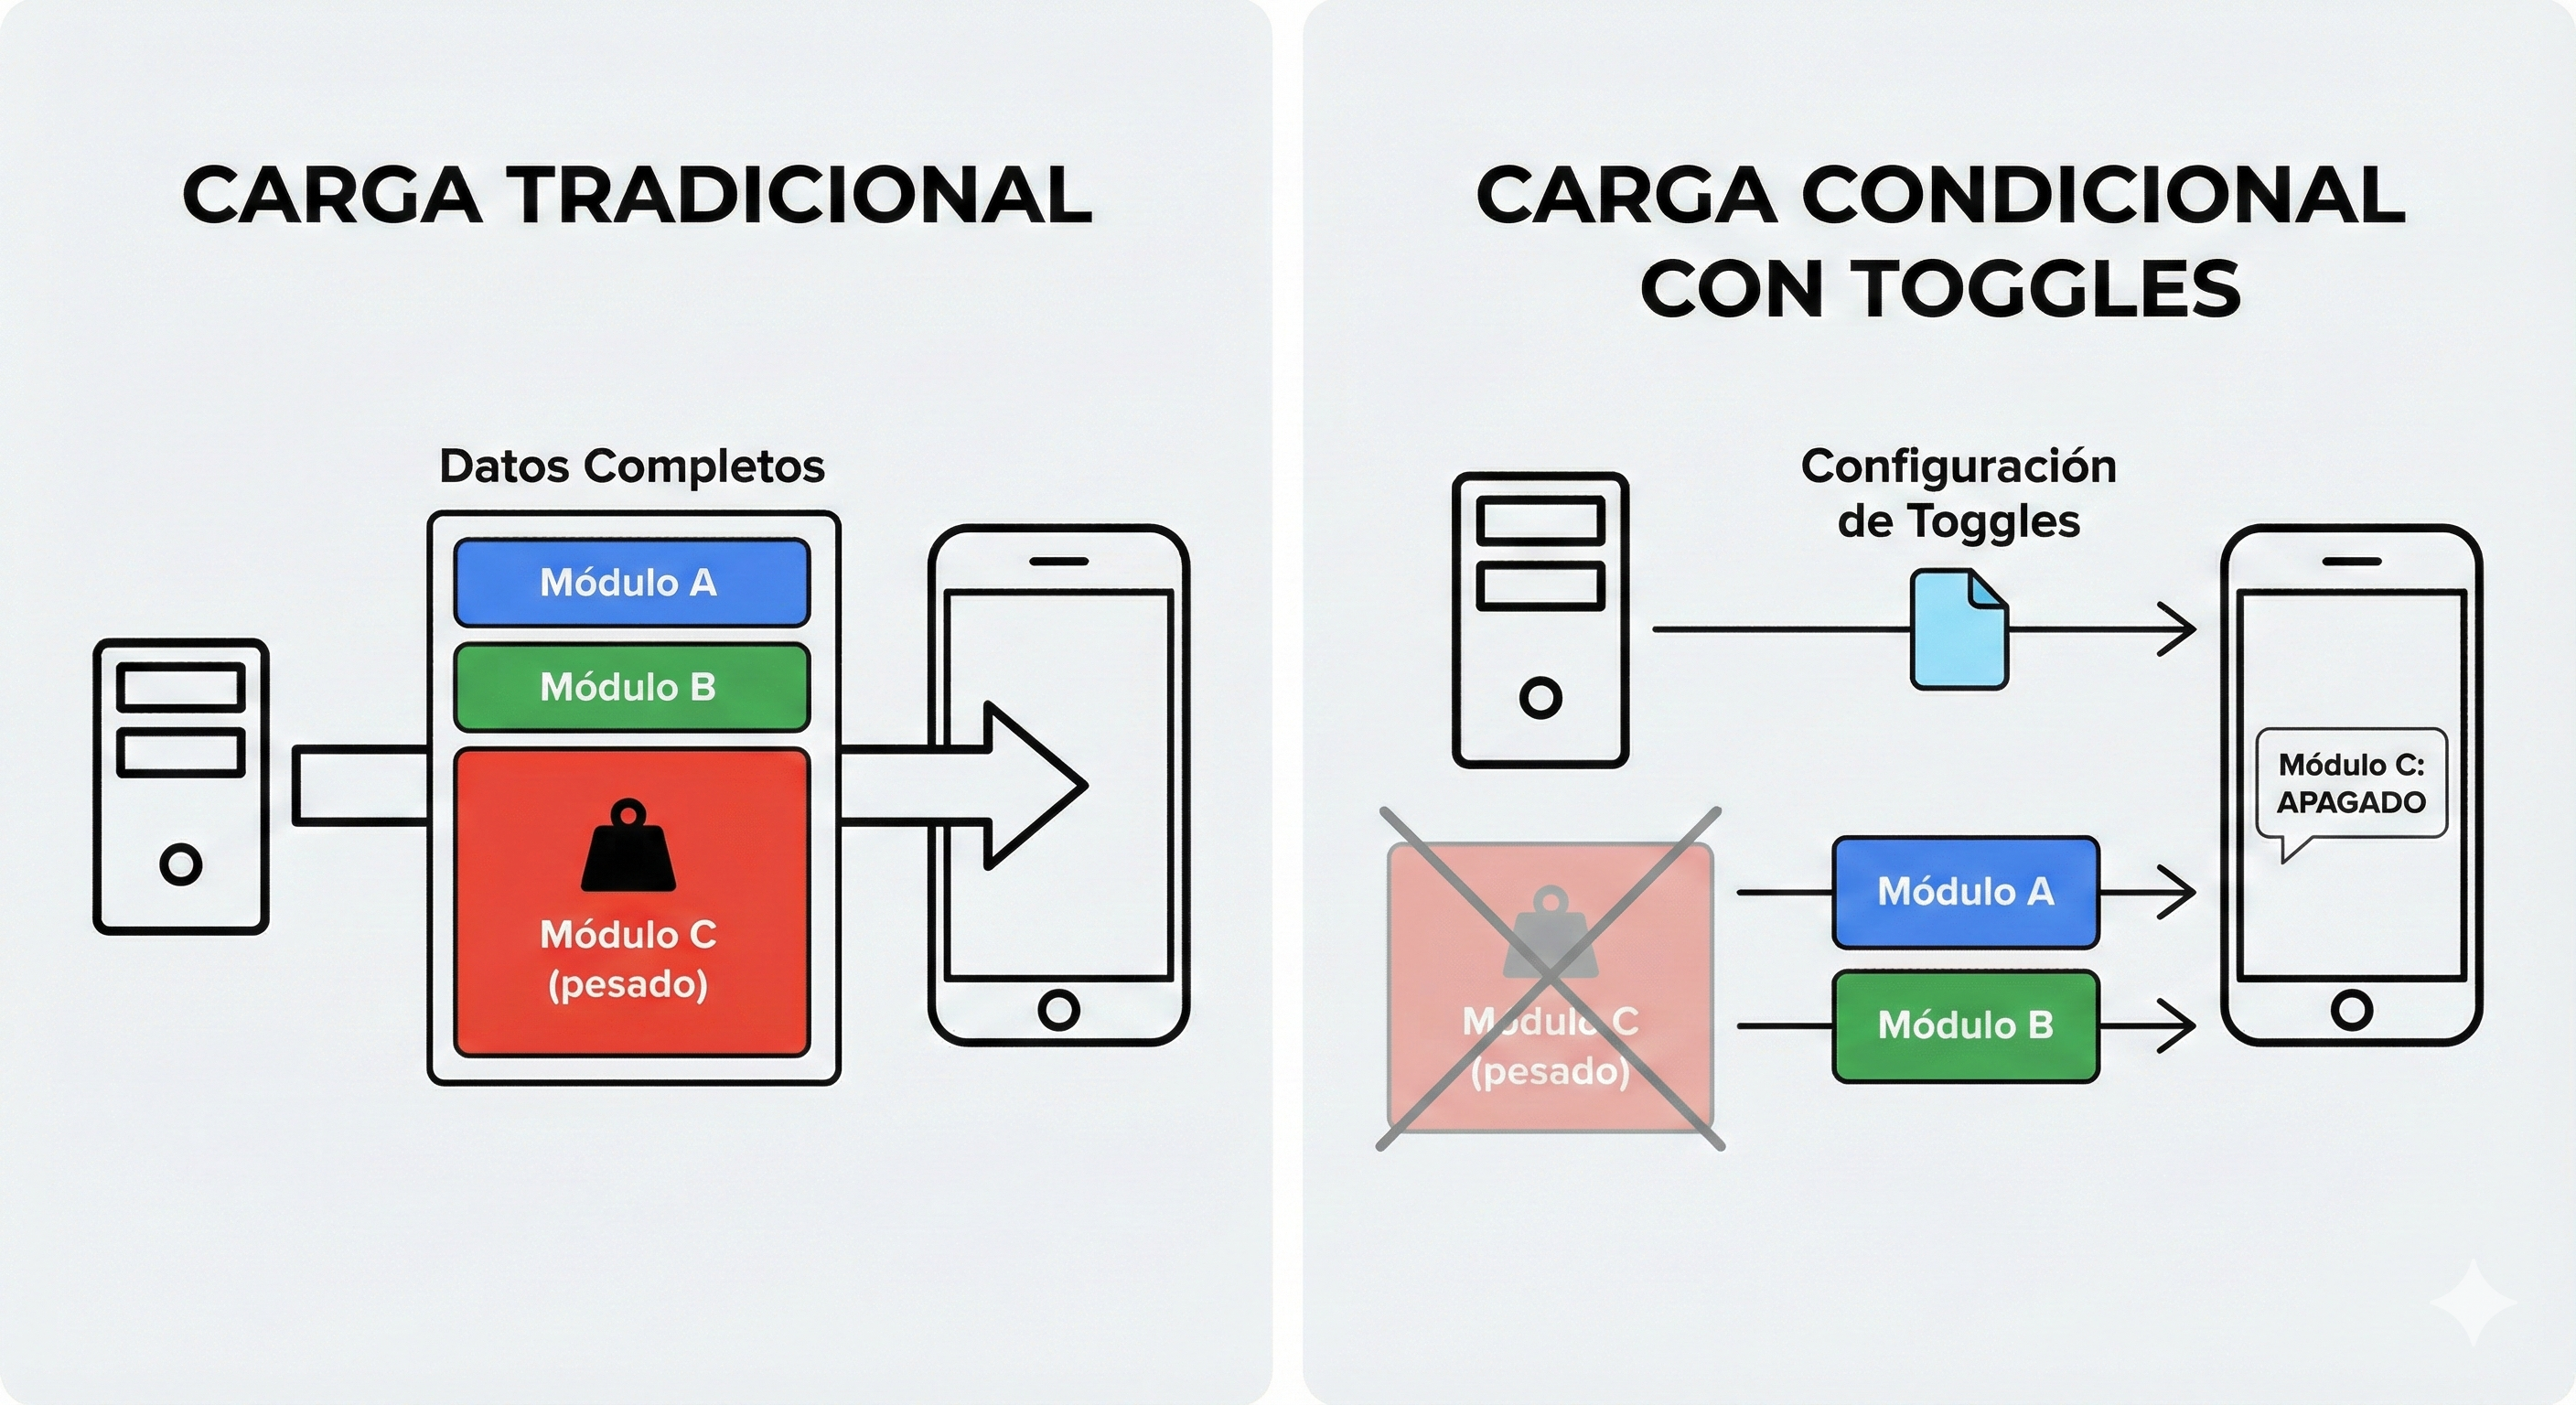
\includegraphics[width=0.9\columnwidth]{graphics/lazy_loading_toggle.png}
    \caption{Comparación del proceso de carga de recursos en el frontend. A la izquierda, la carga tradicional descarga todos los módulos JavaScript. A la derecha, la propuesta de carga condicional impulsada por Feature Toggles.}
    \label{fig:lazy_loading}
\end{figure}

\subsubsection{Manejo de Base de Datos: Patrón Expand--Contract}

Uno de los desafíos más complejos, identificado por \cite{rahman2016msr}, es la gestión de cambios en el esquema de la base de datos. Para resolver esto sin tiempo de inactividad, se adopta el patrón \textbf{Expand--Contract (Parallel Change)}:

\begin{enumerate}
    \item \textbf{Fase Expand:} Se añaden nuevas columnas o tablas sin afectar al código antiguo.
    \item \textbf{Fase Migrate:} Un proceso en segundo plano sincroniza los datos antiguos.
    \item \textbf{Fase Contract:} Se elimina la estructura antigua una vez estabilizada la nueva.
\end{enumerate}

Esta estrategia desacopla la migración de datos del despliegue de la aplicación, eliminando bloqueos de tablas durante actualizaciones.

\subsubsection{Estrategia de Caché y Rendimiento}

Para evitar latencias por consultas repetidas al gestor de toggles, se diseñó una arquitectura de caché de dos niveles:

\begin{itemize}
    \item \textbf{L1 (Memoria):} \texttt{IMemoryCache} con TTL corto (ej. 30 segundos).
    \item \textbf{L2 (Distribuido):} Caché distribuido (Redis) antes de consultar SQL Server.
\end{itemize}

Esta arquitectura garantiza tiempos de respuesta sub-milisegundo, abordando las preocupaciones de rendimiento señaladas por \cite{sharma2024complexity}.
